\chapter{Hình học}

\index{geometry}
\index{hình học}

Trong các bài toán hình học, thường khá thách thức
để tìm ra cách tiếp cận bài toán sao cho
có thể cài đặt lời giải một cách thuận tiện
và số lượng trường hợp đặc biệt là ít.

Ví dụ như xét một bài toán trong đó
ta được cho các đỉnh của một tứ giác
(một đa giác có bốn đỉnh),
và nhiệm vụ của ta là tính diện tích của nó.
Ví dụ, một đầu vào có thể của bài toán như sau:

\begin{center}
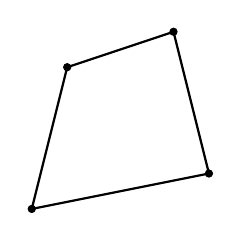
\begin{tikzpicture}[scale=0.45]

\draw[fill] (6,2) circle [radius=0.1];
\draw[fill] (5,6) circle [radius=0.1];
\draw[fill] (2,5) circle [radius=0.1];
\draw[fill] (1,1) circle [radius=0.1];
\draw[thick] (6,2) -- (5,6) -- (2,5) -- (1,1) -- (6,2);
\end{tikzpicture}
\end{center}
Một cách tiếp cận bài toán là chia
tứ giác thành hai tam giác bằng một đường
thẳng nối hai đỉnh đối diện:
\begin{center}
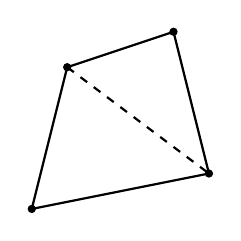
\begin{tikzpicture}[scale=0.45]

\draw[fill] (6,2) circle [radius=0.1];
\draw[fill] (5,6) circle [radius=0.1];
\draw[fill] (2,5) circle [radius=0.1];
\draw[fill] (1,1) circle [radius=0.1];

\draw[thick] (6,2) -- (5,6) -- (2,5) -- (1,1) -- (6,2);
\draw[dashed,thick] (2,5) -- (6,2);
\end{tikzpicture}
\end{center}
Sau đó, chỉ cần tính tổng diện tích
của hai tam giác.
Diện tích của một tam giác có thể được tính,
ví dụ, bằng \key{công thức Heron} (Heron's formula)
%\footnote{Heron of Alexandria (c. 10--70) was a Greek mathematician.}
\[ \sqrt{s (s-a) (s-b) (s-c)},\]
trong đó $a$, $b$ và $c$ là độ dài
các cạnh của tam giác và
$s=(a+b+c)/2$.
\index{Heron's formula}
\index{công thức Heron}

Đây là một cách có thể để giải bài toán,
nhưng có một cạm bẫy:
làm thế nào để chia tứ giác thành các tam giác?
Hóa ra đôi khi ta không thể chỉ chọn 
hai đỉnh đối diện bất kỳ.
Ví dụ, trong tình huống sau,
đường chia nằm \emph{bên ngoài} tứ giác:
\begin{center}
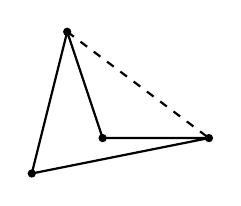
\begin{tikzpicture}[scale=0.45]

\draw[fill] (6,2) circle [radius=0.1];
\draw[fill] (3,2) circle [radius=0.1];
\draw[fill] (2,5) circle [radius=0.1];
\draw[fill] (1,1) circle [radius=0.1];
\draw[thick] (6,2) -- (3,2) -- (2,5) -- (1,1) -- (6,2);

\draw[dashed,thick] (2,5) -- (6,2);
\end{tikzpicture}
\end{center}
Tuy nhiên, một cách vẽ đường khác lại được:
\begin{center}
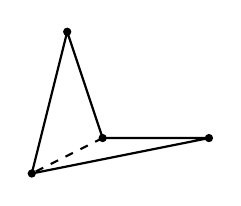
\begin{tikzpicture}[scale=0.45]

\draw[fill] (6,2) circle [radius=0.1];
\draw[fill] (3,2) circle [radius=0.1];
\draw[fill] (2,5) circle [radius=0.1];
\draw[fill] (1,1) circle [radius=0.1];
\draw[thick] (6,2) -- (3,2) -- (2,5) -- (1,1) -- (6,2);

\draw[dashed,thick] (3,2) -- (1,1);
\end{tikzpicture}
\end{center}
Với con người thì rõ ràng đường nào là lựa chọn đúng,
nhưng tình huống này lại khó với máy tính.
                           
Tuy nhiên, hóa ra ta có thể giải quyết bài toán bằng cách dùng
một phương pháp khác thuận tiện hơn cho lập trình viên.
Cụ thể, có một công thức tổng quát
\[x_1y_2-x_2y_1+x_2y_3-x_3y_2+x_3y_4-x_4y_3+x_4y_1-x_1y_4,\]
tính được diện tích của một tứ giác
có các đỉnh là
$(x_1,y_1)$,
$(x_2,y_2)$,
$(x_3,y_3)$ và
$(x_4,y_4)$.
Công thức này dễ cài đặt, không có trường hợp
đặc biệt nào, và ta thậm chí có thể tổng quát hóa công thức này
cho \emph{mọi} đa giác.

\section{Số phức}

\index{complex number}
\index{số phức}
\index{point}
\index{điểm}
\index{vector}
\index{vectơ}

\key{Số phức} (complex number) là số có dạng $x+y i$,
trong đó $i = \sqrt{-1}$ là \key{đơn vị ảo} (imaginary unit).
Một cách diễn giải hình học của số phức là
nó biểu diễn một điểm hai chiều $(x,y)$
hoặc một vectơ từ gốc tọa độ đến điểm $(x,y)$.

Ví dụ, $4+2i$ tương ứng với
điểm và vectơ sau:

\begin{center}
\begin{tikzpicture}[scale=0.45]

\draw[->,thick] (-5,0)--(5,0);
\draw[->,thick] (0,-5)--(0,5);

\draw[fill] (4,2) circle [radius=0.1];
\draw[->,thick] (0,0)--(4-0.1,2-0.1);

\node at (4,2.8) {$(4,2)$};
\end{tikzpicture}
\end{center}

\index{complex@\texttt{complex}}

Lớp số phức \texttt{complex} trong C++ rất
hữu ích khi giải các bài toán hình học.
Sử dụng lớp này ta có thể biểu diễn điểm và vectơ
dưới dạng số phức, và lớp này chứa các công cụ
hữu ích trong hình học.

Trong đoạn mã sau, \texttt{C} là kiểu dữ liệu của
tọa độ và \texttt{P} là kiểu dữ liệu của điểm hoặc vectơ.
Thêm vào đó, đoạn mã định nghĩa các macro \texttt{X} và \texttt{Y}
có thể được sử dụng để tham chiếu đến tọa độ x và y.

\begin{lstlisting}
typedef long long C;
typedef complex<C> P;
#define X real()
#define Y imag()
\end{lstlisting}

Ví dụ, đoạn mã sau định nghĩa một điểm $p=(4,2)$
và in ra tọa độ x và y của nó:

\begin{lstlisting}
P p = {4,2};
cout << p.X << " " << p.Y << "\n"; // 4 2
\end{lstlisting}

Đoạn mã sau định nghĩa các vectơ $v=(3,1)$ và $u=(2,2)$,
và sau đó tính tổng $s=v+u$.

\begin{lstlisting}
P v = {3,1};
P u = {2,2};
P s = v+u;
cout << s.X << " " << s.Y << "\n"; // 5 3
\end{lstlisting}

Trong thực tế,
kiểu dữ liệu tọa độ phù hợp thường là
\texttt{long long} (số nguyên) hoặc \texttt{long double}
(số thực).
Sử dụng số nguyên bất cứ khi nào có thể là một ý tưởng tốt,
vì các phép tính với số nguyên là chính xác.
Nếu cần dùng số thực,
lỗi làm tròn nên được tính đến
khi so sánh các số.
Một cách an toàn để kiểm tra xem các số thực $a$ và $b$ có bằng nhau không
là so sánh chúng bằng cách dùng $|a-b|<\epsilon$,
trong đó $\epsilon$ là một số nhỏ (ví dụ, $\epsilon=10^{-9}$).

\subsubsection*{Các hàm}

Trong các ví dụ sau, kiểu dữ liệu tọa độ là
\texttt{long double}.

Hàm $\texttt{abs}(v)$ tính độ dài
$|v|$ của một vectơ $v=(x,y)$
sử dụng công thức $\sqrt{x^2+y^2}$.
Hàm này cũng có thể được sử dụng để
tính khoảng cách giữa các điểm
$(x_1,y_1)$ và $(x_2,y_2)$,
bởi vì khoảng cách đó bằng độ dài
của vectơ $(x_2-x_1,y_2-y_1)$.

Đoạn mã sau tính khoảng cách
giữa điểm $(4,2)$ và $(3,-1)$:
\begin{lstlisting}
P a = {4,2};
P b = {3,-1};
cout << abs(b-a) << "\n"; // 3.16228
\end{lstlisting}

Hàm $\texttt{arg}(v)$ tính 
góc của một vectơ $v=(x,y)$ so với trục x.
Hàm trả về góc theo radian,
trong đó $r$ radian bằng $180 r/\pi$ độ.
Góc của một vectơ chỉ về phía phải là 0,
và góc giảm theo chiều kim đồng hồ và tăng 
ngược chiều kim đồng hồ.

Hàm $\texttt{polar}(s,a)$ tạo ra một vectơ
có độ dài là $s$ và chỉ về góc $a$.
Một vectơ có thể được xoay một góc $a$
bằng cách nhân nó với một vectơ có độ dài 1 và góc $a$.

Đoạn mã sau tính góc của 
vectơ $(4,2)$, xoay nó $1/2$ radian
ngược chiều kim đồng hồ, và sau đó tính lại góc:

\begin{lstlisting}
P v = {4,2};
cout << arg(v) << "\n"; // 0.463648
v *= polar(1.0,0.5);
cout << arg(v) << "\n"; // 0.963648
\end{lstlisting}

\section{Điểm và đường thẳng}

\index{cross product}
\index{tích có hướng}

\key{Tích có hướng} (cross product) $a \times b$ của các vectơ
$a=(x_1,y_1)$ và $b=(x_2,y_2)$ được tính
bằng công thức $x_1 y_2 - x_2 y_1$.
Tích có hướng cho ta biết liệu $b$
rẽ trái (giá trị dương), không rẽ (bằng không)
hay rẽ phải (giá trị âm)
khi nó được đặt ngay sau $a$.

Hình sau minh họa các trường hợp trên:
\begin{center}
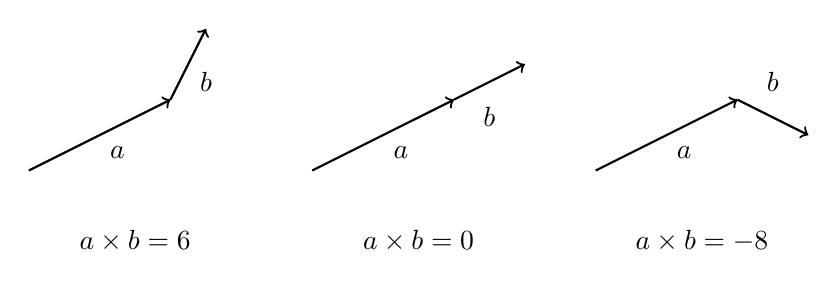
\begin{tikzpicture}[scale=0.45]

\draw[->,thick] (0,0)--(4,2);
\draw[->,thick] (4,2)--(4+1,2+2);

\node at (2.5,0.5) {$a$};
\node at (5,2.5) {$b$};

\node at (3,-2) {$a \times b = 6$};

\draw[->,thick] (8+0,0)--(8+4,2);
\draw[->,thick] (8+4,2)--(8+4+2,2+1);

\node at (8+2.5,0.5) {$a$};
\node at (8+5,1.5) {$b$};

\node at (8+3,-2) {$a \times b = 0$};

\draw[->,thick] (16+0,0)--(16+4,2);
\draw[->,thick] (16+4,2)--(16+4+2,2-1);

\node at (16+2.5,0.5) {$a$};
\node at (16+5,2.5) {$b$};

\node at (16+3,-2) {$a \times b = -8$};
\end{tikzpicture}
\end{center}

\noindent
Ví dụ, trong trường hợp đầu tiên
$a=(4,2)$ và $b=(1,2)$.
Đoạn mã sau tính tích có hướng
sử dụng lớp \texttt{complex}:

\begin{lstlisting}
P a = {4,2};
P b = {1,2};
C p = (conj(a)*b).Y; // 6
\end{lstlisting}

Đoạn mã trên hoạt động vì
hàm \texttt{conj} đổi dấu tọa độ y
của một vectơ,
và khi các vectơ $(x_1,-y_1)$ và $(x_2,y_2)$
được nhân với nhau, tọa độ y
của kết quả là $x_1 y_2 - x_2 y_1$.

\subsubsection{Vị trí điểm}

Tích có hướng có thể được sử dụng để kiểm tra
xem một điểm nằm ở bên trái hay bên phải
của một đường thẳng.
Giả sử đường thẳng đi qua các điểm
$s_1$ và $s_2$, ta đang nhìn từ $s_1$
đến $s_2$ và điểm cần kiểm tra là $p$.

Ví dụ, trong hình sau,
$p$ nằm ở bên trái của đường thẳng:
\begin{center}
\begin{tikzpicture}[scale=0.45]
\draw[dashed,thick,->] (0,-3)--(12,6);
\draw[fill] (4,0) circle [radius=0.1];
\draw[fill] (8,3) circle [radius=0.1];
\draw[fill] (5,3) circle [radius=0.1];
\node at (4,-1) {$s_1$};
\node at (8,2) {$s_2$};
\node at (5,4) {$p$};
\end{tikzpicture}
\end{center}

Tích có hướng $(p-s_1) \times (p-s_2)$
cho ta biết vị trí của điểm $p$.
Nếu tích có hướng dương,
$p$ nằm ở bên trái,
và nếu tích có hướng âm,
$p$ nằm ở bên phải.
Cuối cùng, nếu tích có hướng bằng không,
các điểm $s_1$, $s_2$ và $p$ nằm trên cùng một đường thẳng.

\subsubsection{Giao điểm của đoạn thẳng}

\index{line segment intersection}
\index{giao điểm của đoạn thẳng}

Tiếp theo ta xét bài toán kiểm tra
liệu hai đoạn thẳng
$ab$ và $cd$ có giao nhau không. Các trường hợp có thể xảy ra là:

\textit{Trường hợp 1:}
Các đoạn thẳng nằm trên cùng một đường thẳng
và chúng chồng lên nhau.
Trong trường hợp này, có vô số
giao điểm.
Ví dụ, trong hình sau,
tất cả các điểm giữa $c$ và $b$ là
giao điểm:
\begin{center}
\begin{tikzpicture}[scale=0.9]
\draw (1.5,1.5)--(6,3);
\draw (0,1)--(4.5,2.5);
\draw[fill] (0,1) circle [radius=0.05];
\node at (0,0.5) {$a$};
\draw[fill] (1.5,1.5) circle [radius=0.05];
\node at (6,2.5) {$d$};
\draw[fill] (4.5,2.5) circle [radius=0.05];
\node at (1.5,1) {$c$};
\draw[fill] (6,3) circle [radius=0.05];
\node at (4.5,2) {$b$};
\end{tikzpicture}
\end{center}

Trong trường hợp này, ta có thể sử dụng tích có hướng để
kiểm tra xem tất cả các điểm có nằm trên cùng một đường thẳng không.
Sau đó, ta có thể sắp xếp các điểm và kiểm tra
liệu các đoạn thẳng có chồng lên nhau không.

\textit{Trường hợp 2:}
Các đoạn thẳng có một đỉnh chung
là điểm giao duy nhất.
Ví dụ, trong hình sau
điểm giao là $b=c$:

\begin{center}
\begin{tikzpicture}[scale=0.9]
\draw (0,0)--(4,2);
\draw (4,2)--(6,1);
\draw[fill] (0,0) circle [radius=0.05];
\draw[fill] (4,2) circle [radius=0.05];
\draw[fill] (6,1) circle [radius=0.05];

\node at (0,0.5) {$a$};
\node at (4,2.5) {$b=c$};
\node at (6,1.5) {$d$};
\end{tikzpicture}
\end{center}

Trường hợp này dễ kiểm tra, bởi vì
chỉ có bốn khả năng
cho điểm giao:
$a=c$, $a=d$, $b=c$ và $b=d$.

\textit{Trường hợp 3:}
Có chính xác một giao điểm
không phải là đỉnh của bất kỳ đoạn thẳng nào.
Trong hình sau, điểm $p$
là giao điểm:
\begin{center}
\begin{tikzpicture}[scale=0.9]
\draw (0,1)--(6,3);
\draw (2,4)--(4,0);
\draw[fill] (0,1) circle [radius=0.05];
\node at (0,0.5) {$c$};
\draw[fill] (6,3) circle [radius=0.05];
\node at (6,2.5) {$d$};
\draw[fill] (2,4) circle [radius=0.05];
\node at (1.5,3.5) {$a$};
\draw[fill] (4,0) circle [radius=0.05];
\node at (4,-0.4) {$b$};
\draw[fill] (3,2) circle [radius=0.05];
\node at (3,1.5) {$p$};
\end{tikzpicture}
\end{center}

Trong trường hợp này, các đoạn thẳng giao nhau
khi và chỉ khi cả hai điểm $c$ và $d$ đều
nằm ở hai bên khác nhau của đường thẳng qua $a$ và $b$,
và các điểm $a$ và $b$ nằm ở hai bên khác nhau
của đường thẳng qua $c$ và $d$.
Ta có thể sử dụng tích có hướng để kiểm tra điều này.

\subsubsection{Khoảng cách từ điểm đến đường thẳng}

Một tính chất khác của tích có hướng là
diện tích của một tam giác có thể được tính
bằng công thức
\[\frac{| (a-c) \times (b-c) |}{2},\]
trong đó $a$, $b$ và $c$ là các đỉnh của tam giác.
Sử dụng sự thật này, ta có thể suy ra một công thức
để tính khoảng cách ngắn nhất từ một điểm đến một đường thẳng.
Ví dụ, trong hình sau $d$ là
khoảng cách ngắn nhất giữa điểm $p$ và đường thẳng
được xác định bởi các điểm $s_1$ và $s_2$:
\begin{center}
\begin{tikzpicture}[scale=0.75]
\draw (-2,-1)--(6,3);
\draw[dashed] (1,4)--(2.40,1.2);
\node at (0,-0.5) {$s_1$};
\node at (4,1.5) {$s_2$};
\node at (0.5,4) {$p$};
\node at (2,2.7) {$d$};
\draw[fill] (0,0) circle [radius=0.05];
\draw[fill] (4,2) circle [radius=0.05];
\draw[fill] (1,4) circle [radius=0.05];
\end{tikzpicture}
\end{center}

Diện tích của tam giác có các đỉnh là
$s_1$, $s_2$ và $p$ có thể được tính theo hai cách:
nó vừa bằng
$\frac{1}{2} |s_2-s_1| d$ và
$\frac{1}{2} ((s_1-p) \times (s_2-p))$.
Do đó, khoảng cách ngắn nhất là
\[ d = \frac{(s_1-p) \times (s_2-p)}{|s_2-s_1|} .\]

\subsubsection{Điểm trong đa giác}

Bây giờ ta hãy xét bài toán
kiểm tra xem một điểm nằm bên trong hay bên ngoài
một đa giác.
Ví dụ, trong hình sau điểm $a$
nằm bên trong đa giác và điểm $b$ nằm bên ngoài
đa giác.

\begin{center}
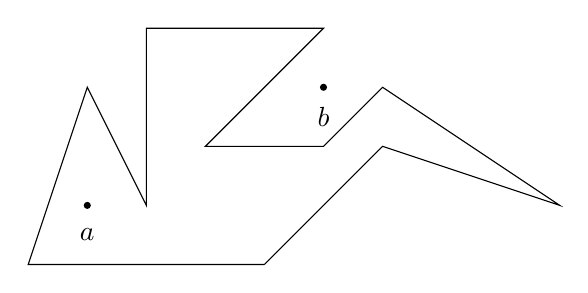
\begin{tikzpicture}[scale=0.75]
%\draw (0,0)--(2,-2)--(3,1)--(5,1)--(2,3)--(1,2)--(-1,2)--(1,4)--(-2,4)--(-2,1)--(-3,3)--(-4,0)--(0,0);
\draw (0,0)--(2,2)--(5,1)--(2,3)--(1,2)--(-1,2)--(1,4)--(-2,4)--(-2,1)--(-3,3)--(-4,0)--(0,0);

\draw[fill] (-3,1) circle [radius=0.05];
\node at (-3,0.5) {$a$};
\draw[fill] (1,3) circle [radius=0.05];
\node at (1,2.5) {$b$};
\end{tikzpicture}
\end{center}

Một cách thuận tiện để giải quyết bài toán là
phóng một \emph{tia} từ điểm đó theo một hướng bất kỳ
và tính số lần nó chạm
vào biên của đa giác.
Nếu số lần là lẻ,
điểm nằm bên trong đa giác,
và nếu số lần là chẵn,
điểm nằm bên ngoài đa giác.

\begin{samepage}
Ví dụ, ta có thể phóng các tia sau:
\begin{center}
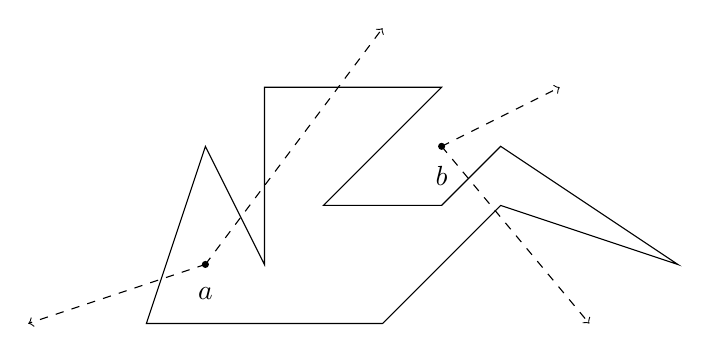
\begin{tikzpicture}[scale=0.75]
\draw (0,0)--(2,2)--(5,1)--(2,3)--(1,2)--(-1,2)--(1,4)--(-2,4)--(-2,1)--(-3,3)--(-4,0)--(0,0);

\draw[fill] (-3,1) circle [radius=0.05];
\node at (-3,0.5) {$a$};
\draw[fill] (1,3) circle [radius=0.05];
\node at (1,2.5) {$b$};

\draw[dashed,->] (-3,1)--(-6,0);
\draw[dashed,->] (-3,1)--(0,5);

\draw[dashed,->] (1,3)--(3.5,0);
\draw[dashed,->] (1,3)--(3,4);
\end{tikzpicture}
\end{center}
\end{samepage}

Các tia từ $a$ chạm biên 1 và 3 lần
biên của đa giác,
nên $a$ nằm bên trong đa giác.
Tương tự, các tia từ $b$
chạm biên 0 và 2 lần,
nên $b$ nằm bên ngoài đa giác.

\section{Diện tích đa giác}

Một công thức tổng quát để tính diện tích
của một đa giác, đôi khi được gọi là \key{công thức dây giày} (shoelace formula),
như sau: \index{shoelace formula}\index{công thức dây giày}
\[\frac{1}{2} |\sum_{i=1}^{n-1} (p_i \times p_{i+1})| =
\frac{1}{2} |\sum_{i=1}^{n-1} (x_i y_{i+1} - x_{i+1} y_i)|, \]
Ở đây các đỉnh là
$p_1=(x_1,y_1)$, $p_2=(x_2,y_2)$, $\ldots$, $p_n=(x_n,y_n)$
theo thứ tự sao cho
$p_i$ và $p_{i+1}$ là các đỉnh liền kề trên biên
của đa giác,
và đỉnh đầu tiên và cuối cùng là cùng một đỉnh, tức là $p_1=p_n$.

Ví dụ, diện tích của đa giác
\begin{center}
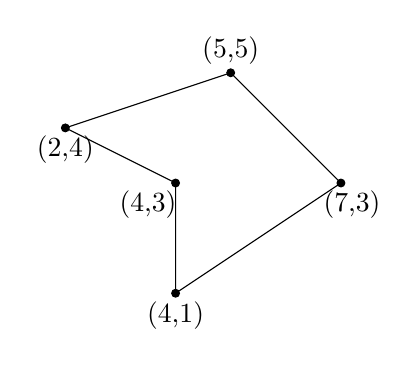
\begin{tikzpicture}[scale=0.7]
\filldraw (4,1.4) circle (2pt);
\filldraw (7,3.4) circle (2pt);
\filldraw (5,5.4) circle (2pt);
\filldraw (2,4.4) circle (2pt);
\filldraw (4,3.4) circle (2pt);
\node (1) at (4,1) {(4,1)};
\node (2) at (7.2,3) {(7,3)};
\node (3) at (5,5.8) {(5,5)};
\node (4) at (2,4) {(2,4)};
\node (5) at (3.5,3) {(4,3)};
\path[draw] (4,1.4) -- (7,3.4) -- (5,5.4) -- (2,4.4) -- (4,3.4) -- (4,1.4);
\end{tikzpicture}
\end{center}
là
\[\frac{|(2\cdot5-5\cdot4)+(5\cdot3-7\cdot5)+(7\cdot1-4\cdot3)+(4\cdot3-4\cdot1)+(4\cdot4-2\cdot3)|}{2} = 17/2.\]

Ý tưởng của công thức là đi qua các hình thang
mà một cạnh là cạnh của đa giác,
và cạnh kia nằm trên đường nằm ngang $y=0$.
Ví dụ:
\begin{center}
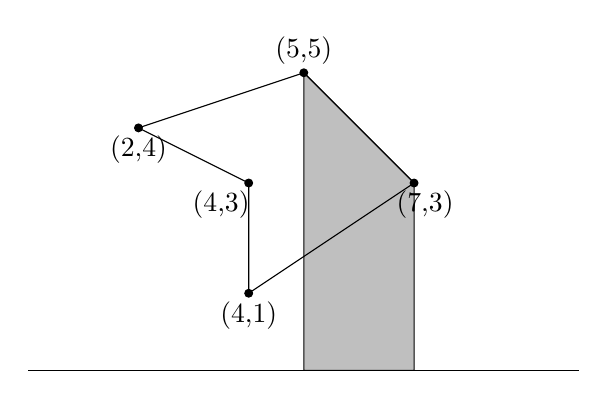
\begin{tikzpicture}[scale=0.7]
\path[draw,fill=lightgray] (5,5.4) -- (7,3.4) -- (7,0) -- (5,0) -- (5,5.4);
\filldraw (4,1.4) circle (2pt);
\filldraw (7,3.4) circle (2pt);
\filldraw (5,5.4) circle (2pt);
\filldraw (2,4.4) circle (2pt);
\filldraw (4,3.4) circle (2pt);
\node (1) at (4,1) {(4,1)};
\node (2) at (7.2,3) {(7,3)};
\node (3) at (5,5.8) {(5,5)};
\node (4) at (2,4) {(2,4)};
\node (5) at (3.5,3) {(4,3)};
\path[draw] (4,1.4) -- (7,3.4) -- (5,5.4) -- (2,4.4) -- (4,3.4) -- (4,1.4);
\draw (0,0) -- (10,0);
\end{tikzpicture}
\end{center}
Diện tích của một hình thang như vậy là
\[(x_{i+1}-x_{i}) \frac{y_i+y_{i+1}}{2},\]
trong đó các đỉnh của đa giác là $p_i$ và $p_{i+1}$.
Nếu $x_{i+1}>x_{i}$, diện tích dương,
và nếu $x_{i+1}<x_{i}$, diện tích âm.

Diện tích của đa giác là tổng diện tích của
tất cả các hình thang như vậy, cho ta công thức
\[|\sum_{i=1}^{n-1} (x_{i+1}-x_{i}) \frac{y_i+y_{i+1}}{2}| =
\frac{1}{2} |\sum_{i=1}^{n-1} (x_i y_{i+1} - x_{i+1} y_i)|.\]

Lưu ý rằng giá trị tuyệt đối của tổng được lấy,
bởi vì giá trị của tổng có thể dương hoặc âm,
phụ thuộc vào việc ta đi theo chiều kim đồng hồ hay ngược chiều kim đồng hồ
dọc theo biên của đa giác.

\subsubsection{Định lý Pick}

\index{Pick's theorem}
\index{định lý Pick}

\key{Định lý Pick} (Pick's theorem) cung cấp một cách khác để tính
diện tích của một đa giác nếu tất cả các đỉnh
của đa giác có tọa độ nguyên.
Theo định lý Pick, diện tích của đa giác là
\[ a + b/2 -1,\]
trong đó $a$ là số điểm nguyên bên trong đa giác
và $b$ là số điểm nguyên trên biên của đa giác.

Ví dụ, diện tích của đa giác
\begin{center}
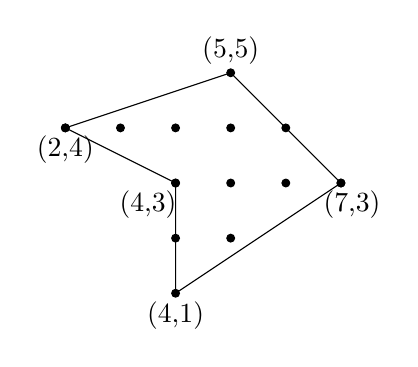
\begin{tikzpicture}[scale=0.7]
\filldraw (4,1.4) circle (2pt);
\filldraw (7,3.4) circle (2pt);
\filldraw (5,5.4) circle (2pt);
\filldraw (2,4.4) circle (2pt);
\filldraw (4,3.4) circle (2pt);
\node (1) at (4,1) {(4,1)};
\node (2) at (7.2,3) {(7,3)};
\node (3) at (5,5.8) {(5,5)};
\node (4) at (2,4) {(2,4)};
\node (5) at (3.5,3) {(4,3)};
\path[draw] (4,1.4) -- (7,3.4) -- (5,5.4) -- (2,4.4) -- (4,3.4) -- (4,1.4);

\filldraw (2,4.4) circle (2pt);
\filldraw (3,4.4) circle (2pt);
\filldraw (4,4.4) circle (2pt);
\filldraw (5,4.4) circle (2pt);
\filldraw (6,4.4) circle (2pt);

\filldraw (4,3.4) circle (2pt);
\filldraw (5,3.4) circle (2pt);
\filldraw (6,3.4) circle (2pt);
\filldraw (7,3.4) circle (2pt);

\filldraw (4,2.4) circle (2pt);
\filldraw (5,2.4) circle (2pt);
\end{tikzpicture}
\end{center}
là $6+7/2-1=17/2$.

\section{Hàm khoảng cách}

\index{distance function}
\index{hàm khoảng cách}
\index{Euclidean distance}
\index{khoảng cách Euclid}
\index{Manhattan distance}
\index{khoảng cách Manhattan}

Một \key{hàm khoảng cách} (distance function) định nghĩa khoảng cách giữa
hai điểm.
Hàm khoảng cách thông dụng nhất là
\key{khoảng cách Euclid} (Euclidean distance) trong đó khoảng cách giữa
các điểm $(x_1,y_1)$ và $(x_2,y_2)$ là
\[\sqrt{(x_2-x_1)^2+(y_2-y_1)^2}.\]
Một hàm khoảng cách khác là
\key{khoảng cách Manhattan} (Manhattan distance)
trong đó khoảng cách giữa các điểm
$(x_1,y_1)$ và $(x_2,y_2)$ là
\[|x_1-x_2|+|y_1-y_2|.\]
\begin{samepage}
Ví dụ, xét hình sau:
\begin{center}
\begin{tikzpicture}

\draw[fill] (2,1) circle [radius=0.05];
\draw[fill] (5,2) circle [radius=0.05];

\node at (2,0.5) {$(2,1)$};
\node at (5,1.5) {$(5,2)$};

\draw[dashed] (2,1) -- (5,2);

\draw[fill] (5+2,1) circle [radius=0.05];
\draw[fill] (5+5,2) circle [radius=0.05];

\node at (5+2,0.5) {$(2,1)$};
\node at (5+5,1.5) {$(5,2)$};

\draw[dashed] (5+2,1) -- (5+2,2);
\draw[dashed] (5+2,2) -- (5+5,2);

\node at (3.5,-0.5) {Khoảng cách Euclid};
\node at (5+3.5,-0.5) {Khoảng cách Manhattan};
\end{tikzpicture}
\end{center}
\end{samepage}
Khoảng cách Euclid giữa hai điểm là
\[\sqrt{(5-2)^2+(2-1)^2}=\sqrt{10}\]
và khoảng cách Manhattan là
\[|5-2|+|2-1|=4.\]
Hình sau thể hiện các vùng có khoảng cách không lớn hơn 1
từ điểm trung tâm, sử dụng khoảng cách Euclid và khoảng cách Manhattan:
\begin{center}
\begin{tikzpicture}

\draw[fill=gray!20] (0,0) circle [radius=1];
\draw[fill] (0,0) circle [radius=0.05];

\node at (0,-1.5) {Khoảng cách Euclid};

\draw[fill=gray!20] (5+0,1) -- (5-1,0) -- (5+0,-1) -- (5+1,0) -- (5+0,1);
\draw[fill] (5,0) circle [radius=0.05];
\node at (5,-1.5) {Khoảng cách Manhattan};
\end{tikzpicture}
\end{center}

\subsubsection{Xoay tọa độ}

Một số bài toán dễ giải hơn nếu
sử dụng khoảng cách Manhattan thay vì khoảng cách Euclid.
Ví dụ, xét bài toán mà trong đó ta được cho
$n$ điểm trên mặt phẳng hai chiều
và nhiệm vụ của ta là tính khoảng cách Manhattan
lớn nhất giữa hai điểm bất kỳ.

Ví dụ, xét tập điểm sau:
\begin{center}
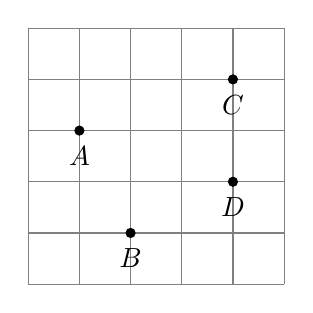
\begin{tikzpicture}[scale=0.65]
\draw[color=gray] (-1,-1) grid (4,4);

\filldraw (0,2) circle (2.5pt);
\filldraw (3,3) circle (2.5pt);
\filldraw (1,0) circle (2.5pt);
\filldraw (3,1) circle (2.5pt);

\node at (0,1.5) {$A$};
\node at (3,2.5) {$C$};
\node at (1,-0.5) {$B$};
\node at (3,0.5) {$D$};
\end{tikzpicture}
\end{center}
Khoảng cách Manhattan lớn nhất là 5
giữa các điểm $B$ và $C$:
\begin{center}
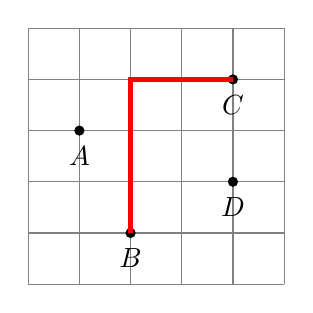
\begin{tikzpicture}[scale=0.65]
\draw[color=gray] (-1,-1) grid (4,4);

\filldraw (0,2) circle (2.5pt);
\filldraw (3,3) circle (2.5pt);
\filldraw (1,0) circle (2.5pt);
\filldraw (3,1) circle (2.5pt);

\node at (0,1.5) {$A$};
\node at (3,2.5) {$C$};
\node at (1,-0.5) {$B$};
\node at (3,0.5) {$D$};

\path[draw=red,thick,line width=2pt] (1,0) -- (1,3) -- (3,3);
\end{tikzpicture}
\end{center}

Một kỹ thuật hữu ích liên quan đến khoảng cách Manhattan
là xoay tất cả các tọa độ 45 độ sao cho
một điểm $(x,y)$ trở thành $(x+y,y-x)$.
Ví dụ, sau khi xoay các điểm trên,
kết quả là:

\begin{center}
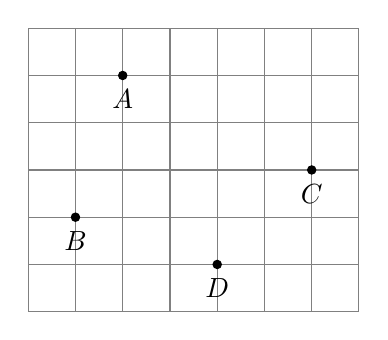
\begin{tikzpicture}[scale=0.6]
\draw[color=gray] (0,-3) grid (7,3);

\filldraw (2,2) circle (2.5pt);
\filldraw (6,0) circle (2.5pt);
\filldraw (1,-1) circle (2.5pt);
\filldraw (4,-2) circle (2.5pt);

\node at (2,1.5) {$A$};
\node at (6,-0.5) {$C$};
\node at (1,-1.5) {$B$};
\node at (4,-2.5) {$D$};
\end{tikzpicture}
\end{center}
Và khoảng cách lớn nhất như sau:
\begin{center}
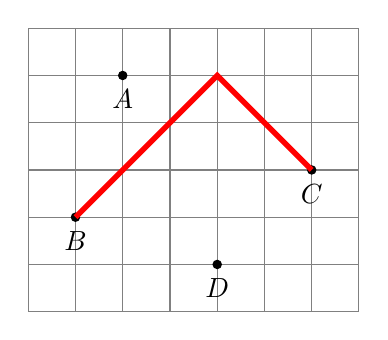
\begin{tikzpicture}[scale=0.6]
\draw[color=gray] (0,-3) grid (7,3);

\filldraw (2,2) circle (2.5pt);
\filldraw (6,0) circle (2.5pt);
\filldraw (1,-1) circle (2.5pt);
\filldraw (4,-2) circle (2.5pt);

\node at (2,1.5) {$A$};
\node at (6,-0.5) {$C$};
\node at (1,-1.5) {$B$};
\node at (4,-2.5) {$D$};

\path[draw=red,thick,line width=2pt] (1,-1) -- (4,2) -- (6,0);
\end{tikzpicture}
\end{center}

Xét hai điểm $p_1=(x_1,y_1)$ và $p_2=(x_2,y_2)$ có tọa độ sau khi xoay
là $p'_1=(x'_1,y'_1)$ và $p'_2=(x'_2,y'_2)$.
Bây giờ có hai cách để biểu diễn khoảng cách Manhattan
giữa $p_1$ và $p_2$:
\[|x_1-x_2|+|y_1-y_2| = \max(|x'_1-x'_2|,|y'_1-y'_2|)\]

Ví dụ, nếu $p_1=(1,0)$ và $p_2=(3,3)$,
các tọa độ sau khi xoay là $p'_1=(1,-1)$ và $p'_2=(6,0)$
và khoảng cách Manhattan là
\[|1-3|+|0-3| = \max(|1-6|,|-1-0|) = 5.\]

Các tọa độ sau khi xoay cung cấp một cách đơn giản
để làm việc với khoảng cách Manhattan, bởi vì ta có thể
xét tọa độ x và y một cách riêng biệt.
Để tối đa hóa khoảng cách Manhattan giữa hai điểm,
ta nên tìm hai điểm mà
tọa độ sau khi xoay của chúng làm tối đa giá trị
\[\max(|x'_1-x'_2|,|y'_1-y'_2|).\]
Điều này dễ dàng, bởi vì hoặc độ chênh lệch theo chiều ngang hoặc theo chiều dọc
của các tọa độ sau khi xoay phải là lớn nhất.
